\documentclass[11pt,compress,t,notes=noshow, aspectratio=169, xcolor=table]{beamer}

\usepackage{../../style/lmu-lecture}
% Defines macros and environments
\input{../../style/common.tex}

\title{Applied Machine Learning}
% \author{LMU}
%\institute{\href{https://compstat-lmu.github.io/lecture_iml/}{compstat-lmu.github.io/lecture\_iml}}
\date{}

\begin{document}

\newcommand{\titlefigure}{figure/performance_vs_interpretability}
\newcommand{\learninggoals}{
\item The Hyperparameter Optimization Problem
\item Grid Search, Random Search and Bayesian optimization
\item Separation of Train and Test}

\lecturechapter{Hyperparameter Tuning}
\lecture{Applied Machine Learning}

\section{Hyperparameter Optimization}
\subsection{Motivation}

% Contains 1-8
\includepdf[pages={2-8}]{i2ml/slides-tuning-nutshell.pdf}

\begin{frame}{The Problem Statement}
\begin{itemize}
\setlength\itemsep{1em}
    \item 
\end{itemize}
    
\end{frame}
\begin{frame}{Parameters vs Hyperparameters}

There is a multitude of technical aspects we need to consider:
\vspace{1em}
\begin{itemize}
\setlength\itemsep{1em}
    \item \textbf{Model type:} 
\end{itemize}
\end{frame}

\begin{frame}{Hyperparameter Types}

\begin{itemize}
\setlength\itemsep{2em}
    \item 
\end{itemize}
\end{frame}

\begin{frame}{Conditional Hyperparameters}

\begin{itemize}
\setlength\itemsep{2em}
    \item 
\end{itemize}
\end{frame}

\begin{frame}{The Untouched Test Set Principle}

\begin{itemize}
\setlength\itemsep{2em}
    \item 
\end{itemize}
\end{frame}

\begin{frame}{Train-Valid-Test Protocol}

\begin{itemize}
\setlength\itemsep{2em}
    \item 
\end{itemize}
\end{frame}

\begin{frame}{Nested Cross-Validation}

\begin{itemize}
\setlength\itemsep{2em}
    \item 
\end{itemize}
\end{frame}

\begin{frame}{Most important factor in ML: correct CV}

\begin{itemize}
\setlength\itemsep{2em}
    \item 
\end{itemize}
\end{frame}

\begin{frame}{Learn operations only on the training set}

\begin{itemize}
\setlength\itemsep{2em}
    \item 
\end{itemize}
\end{frame}

\endlecture
\end{document}
